%S_parameter

Scattering parameters or S-parameters are widely used to describe the electrical behavior of a linear electrical networks. An electrical network can be considered as a 'black box', which contains amounts of interconnected basic electrical circuit components such as  resistors, capacitors, inductors and transistors etc. On this 'black box' may exist many ports, which presented the entries or exits of the networks. 
.
Agilent\cite{aglient_s_parameters} explains the S-Parameter with a 2-port network. Following is s simplest 2-Port network.
\begin{figure}
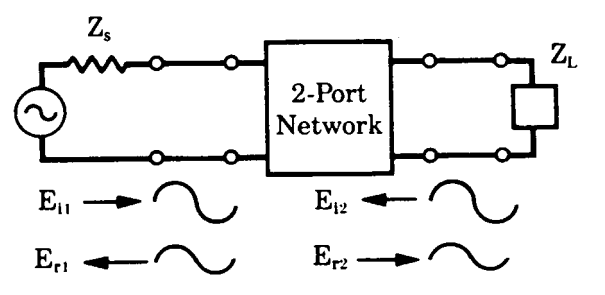
\includegraphics[width=0.4\textwidth]{bilder/s_parameters}
\caption{2-Port-Network \cite{aglient_s_parameters}}
\label{fig:2_port_network}
\end{figure}
$E_{i1}$ and $E_{i2}$ represent the input waves over left and right ports of the network respectively. $E_{r1}$ and $E_{r2}$ are the response from the combination of two input signals $E_{i1}$ and $E_{i2}$. $E_{i1}$ and $E_{r1}$ locate at the same side of the network, so are $E_{i2}$ and $E_{r2}$. Their relation can  be expressed in terms of H-Parameters: 
\begin{align}
E_{r1}&=f_{11}(h)E_{i1}+f_{12}(h)E_{i2}
\label{eq:er1}
\\
E_{r2}&=f_{21}(h)E_{i1}+f_{22}(h)E_{i2}
\label{eq:er2}
\end{align}
Here $f11,f12,f21,f22$ are the network parameters, which indicate the relation between traveling voltages waves  and total voltages or currents. Divied both sides of the functions(\ref{eq:er1}-\ref{eq:er2}) by $\sqrt{Z_{0}}$( $Z_{0}$ System system impedance).A new set of variables are defined:
\begin{align} 
a1&=\frac{Ei1}{\sqrt{Z_{0}}} \quad a2=\frac{Ei2}{\sqrt{Z_{0}}}\\
b1&=\frac{Er1}{\sqrt{Z_{0}}} \quad b2=\frac{Er2}{\sqrt{Z_{0}}}
\end{align}
So relation of the new variables are give by:
\begin{align}
b_{1}&=S_{11}a_{1}+S_{12}a_{2}\\
b_{2}&=S_{21}a_{1}+S_{22}a_{2}
\end{align}
or in matrics form:
\begin{equation}
		\begin{pmatrix}
			b_{1}&\\
			b_{2}&
		\end{pmatrix}
	=	
		\begin{pmatrix}
			S_{11}&S_{12}\\
			S_{21}&S_{22}
		\end{pmatrix}
		\begin{pmatrix}
			a_{1}&\\
			a_{2}&
		\end{pmatrix}
\label{eq:s_matrix}
\end{equation}

The S-Parameters are defined as following:
\begin{align}
S_{11}&=\frac{b_{1}}{a_{1}}|_{a_{2}=0}\\
S_{21}&=\frac{b_{2}}{a_{1}}|_{a_{2}=0}\\
S_{22}&=\frac{b_{2}}{a_{2}}|_{a_{1}=0}\\
S_{12}&=\frac{b_{1}}{a_{2}}|_{a_{1}=0}
\end{align}
This S-Parameter Matrix is described:
\begin{itemize}
\item $S_{11}$ is the input port reflection coefficient
\item $S_{12}$ is the reverse gain
\item $S_{21}$ is the forward gain
\item $S_{22}$ is the output port reflection coefficient
\end{itemize}
In another hand, $S_{21}$ is often used to estimate the transmission ability of a network. Therefore the $S_{21}$ help us to observe the coupling efficiency in this article.
